\subsection{UC7 - Inserimento recensione}\label{usecase:7}
\begin{figure}[H]
  \centering
  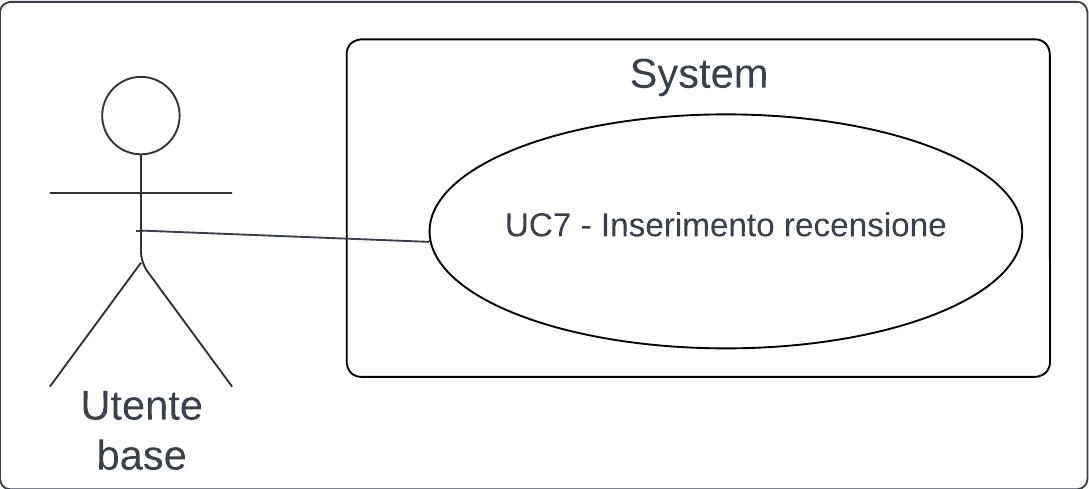
\includegraphics[width=0.7\textwidth]{ucd/UCD7.png}
  \caption{Inserimento recensione}
\end{figure}
\textbf{Attori}:
\begin{itemize}
    \item Utente base.
\end{itemize}
\textbf{Precodizioni}:
\begin{itemize}
    \item L'utente ha selezionato un ristorante dove lasciare la recensione.
\end{itemize}
\textbf{Postcondizioni}:
\begin{itemize}
    \item L'utente rilascia una recensione al ristorante selezionato.
\end{itemize}
\textbf{Scenario principale}:
\begin{enumerate}
    \item L'utente rilascia la recensione sotto forma di numero di stelle su 5 disponibili e con aggiunta di testo;
    \item L'utente conferma la sua recensione.
\end{enumerate}
\textbf{Scenari alternativi}:
\begin{enumerate}
    \item Se la recensione è:
    \begin{enumerate}
        \item Troppo lunga;
        \item Vuota;
    \end{enumerate}
    \item Visualizza un errore;
    \item L'utente deve aggiornare la recensione in modo tale che rispetta i criteri per poterla pubblicare.
\end{enumerate}
\newpage